
\chapter{Champs et masse d'une particule chargée}%TD n°5
\section{Champs d'une particule chargée en mouvement}%1 
On considère une particule de charge q en mouvement rectiligne uniforme à la vitesse {\bf v} par
rapport au référentiel du laboratoire K . Conformément aux notations de la figure 1, on s'intéresse
aux champs créés par la particule $q$ au point $M (x, y, z)$ à l'instant $t$ où la charge $q$ est à la distance $vt$ de $O$.
\begin{center}
 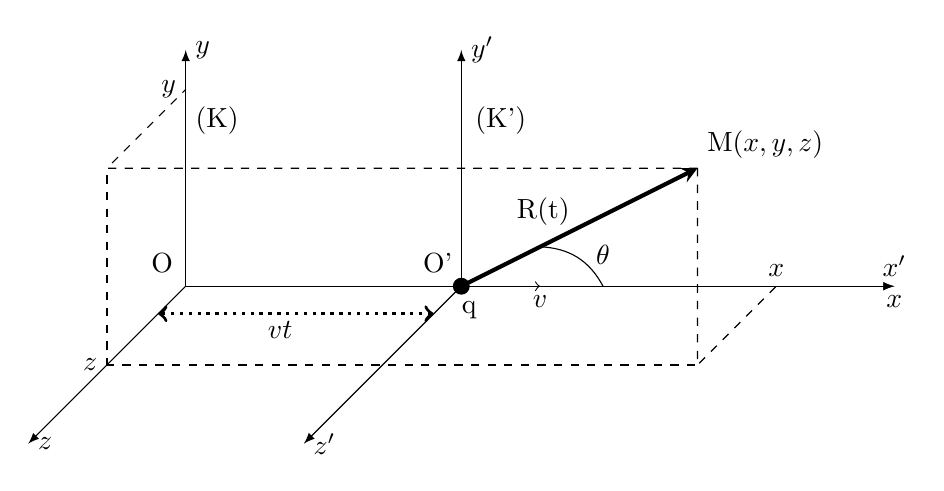
\begin{tikzpicture}[scale=1]
   \coordinate (M) at (3,1.5);
   \coordinate (O) at (0,0);
% Repère K
   \draw [->,-latex] (-3.5,0) --++ (-2,-2) node [right] {$z$};
   \draw [->,-latex] (-3.5,0) --++ (9,0) node [below] {$x$};
   \draw [->,-latex] (-3.5,0) --++ (0,3) node [right] {$y$};
   \node at (-3.8,0.3) {O};
   \node at (-3.1,2.1) {(K)};
% Repère K'
   \draw [->,-latex] (0,0) --++ (-2,-2) node [right] {$z'$};
   \draw [->,-latex] (0,0) --++ (5.5,0) node [above] {$x'$};
   \draw [->,-latex] (0,0) --++ (0,3) node [right] {$y'$};
   \node at (-0.3,0.3){O'};
   \node at (0.5,2.1){(K')};
   \draw [<->, dotted, very thick] (-0.35,-0.35) -- (-3.85,-0.35);%\draw []
   \node at (-2.3,-0.55) {$vt$};
% Particule
   \node at (0.1,-0.3){q};
   \filldraw [black] (0,0) circle (0.1cm);
   \draw [->] (0,0) --++ (1,0) node [below] {$v$}	;
% Vecteur OM
 	\draw [line width=1.5pt,-stealth] (O) -- (M);
    \node at (M) [above right]{M$(x,y,z)$};
    \node at (1.5,0.65) [above left]{\bi{R}(t)};
    \draw (1,0.5) to [bend left] (1.8,0);
    \node at (1.8,0.4) [] {$\theta$};
% Pointillé
    % Vers le bas
 	\draw[dashed] (M) --++ (0,-2.5) --++ (1,1) node [above] {$x$};
 	\draw[dashed] (M) --++ (0,-2.5) --++ (-7.5,0);
 	% Vers l'arrière
 	\draw[dashed] (M) --++ (-7.5,0) --++ (1,1) node [left] {$y$};
 	\draw[dashed] (M) --++ (-7.5,0) --++ (0,-2.5) node [left] {$z$};
 \end{tikzpicture}

Figure 1: Charge en mouvement.
\end{center}
\begin{enumerate}
  \item Calculer les composantes du quadrivecteur potentiel $\wtt{A}$ dans le référentiel K.
  \item En déduire l'expression des champs {\bf }E et {\bf }B au point M en fonction de $q$, $v$, \bi{R} $=$ {\bf O'M} et
$\theta$ , l'angle entre \bi{R} et l'axe des abscisses.
  \item Dessiner les lignes du champ {\bf E} et préciser la limite non relativiste des expressions trouvées
à la question précédente.
\setcounter{numero}{\theenumi}\end{enumerate}
On considère maintenant deux charges identiques, espacées d'une distance a , se déplaçant à la
même vitesse, parallèlement à l'axe $Ox$ (droites d'équations $y=0$ et $y=a$ ).
\begin{enumerate}
  \setcounter{enumi}{\thenumero}
  \item On se place dans le référentiel K. À l'aide des expressions précédentes, montrer que la force
de Lorentz exercée par la charge située sur l'axe ($Ox$) sur l'autre charge s'écrit :
\[
{\bf F}=\frac{}{4\pi\epsilon_0a^2}\sqrt{1-\frac{v^2}{c^2}}{\bf e_y}
\]
  \item Dans l'approximation des faibles vitesses, montrer que cette force se compose d'une force
répulsive et d'une force attractive que l'on interprètera.
\end{enumerate}
\section{Masse électromagnétique}%2 
On modélise une particule chargée par une sphère de rayon a dont la charge q est répartie en
surface.
\begin{enumerate}
  \item On considère tout d'abord la charge immobile. Calculer la densité d'énergie du champ
électromagnétique puis l'énergie totale U 0 du champ. On pourra poser $e^2 = q^2/4\pi\epsilon_0$.
\setcounter{numero}{\theenumi}\end{enumerate}
La particule chargée est maintenant animée d'une vitesse v par rapport au référentiel du
laboratoire (voir Fig. 1).
\begin{enumerate}
  \setcounter{enumi}{\thenumero}
  \item Montrer que l'énergie U et la quantité de mouvement P x du champ dans le référentiel du
laboratoire sont données par les expressions suivantes :
\[
U=\gamma(1+\frac{\beta^2}{3})U' \tag{1}
\] 
\begin{equation}
    P_x=\frac{4U'}{3c^2}\gamma v \tag{2}
\end{equation}
  \item À l'aide de l'expression (2), définir une masse électromagnétique de la particule chargée
notée $m_\tx{élec}$.
  \item Peut-on identifier les expressions (1) et (2) au quadrivecteur énergie-impulsion de la particule dans le référentiel du laboratoire ?
\end{enumerate}
